\chapter{Hashing}
\label{ch:hash}
\label{ch:hashing}

\begin{quote}
{\bf hash:} transitive verb\footnote{Merriam Websters}
\begin{enumerate}
\item
\begin{enumerate}
\item
to chop (as meat and potatoes) into small pieces
\item
confuse, muddle
\end{enumerate}
\item ...
\end{enumerate}
\end{quote}

This is the definition of hash from which the computer term was
derived.  The idea of hashing as originally conceived was to take
values and to chop and mix them to the point that the original values
are muddled.  The term as used in computer science dates back to the
early 1950's.

More formally the idea of hashing is to approximate a random function
$h : \alpha \rightarrow \beta$ from a source (or universe) set $U$ of
type $\alpha$ to a
destination set of type $\beta$.  Most often the source set is significantly
larger than the destination set, so the function not only chops and
mixes but also reduces.  In fact the source set might have infinite
size, such as all character strings, while the destination set always
has finite size.  Also the source set might consist of complicated
elements, such as the set of all directed graphs, while the
destination are typically the integers in some fixed range.  Hash
functions are therefore many to one functions.

Using an actual randomly selected function from the set of all
functions from $\alpha$ to $\beta$ is typically not practical due to
the number of such functions and hence the size (number of bits)
needed to represent such a function.  Therefore in practice one uses
some pseudorandom function.

\begin{exercise}
How many hash functions are there that map from a source set of size $n$
to the integers from 1 to $m$?   How many bits does it take to represent
them?   What if the source set consists of character strings of length
up to 20? Assume there are 100 possible characters.
\end{exercise}

Why is it useful to have random or pseudo random functions that map
from some large set to a smaller set?  Generally such functions might
be used to hide data, to reorder data in a random order, or to spread
data smoothly over a range.
Here we consider some applications of
each.

\begin{enumerate}

\item We saw how hashing can be used in treaps.  In particular we
  suggested using a hash function to hash the keys to generate the
  ``random'' priorities.  Here what was important is that the ordering
  of the priorities is somehow random with respect to the keys.  Our
  analysis assumed the priorities were truly random, but it can be
  shown that a limited form of randomness that arise out of relatively
  simple hash functions is sufficient.

\item
  In cryptography hash functions can be used to hide information.  One
  such application is in digital signatures where a so-called secure
  hash is used to describe a large document with a small number of
  bits.

\item A one-way hash function is used to hide a string, for example
  for password protection.  Instead of storing passwords in plain
  text, only the hash of the password is stored.  To verify whether a
  password entered is correct, the hash of the password is compared to
  the stored value.  These signatures can be used to
  \emph{authenticate} the source of the document, ensure the
  \emph{integrity} of the document as any change to the document
  invalidates the signature, and prevent \emph{repudiation} where the
  sender denies signing the document.

\item String commitment protocols use hash functions to hide to what
  string a sender has committed so that the receiver gets no
  information.  Later, the sender sends a key that allows the receiver
  to reveal the string.  In this way, the sender cannot change the
  string once it is committed, and the receiver can verify that the
  revealed string is the committed string.  Such protocols might be
  used to flip a coin across the Internet: The sender flips a coin and
  commits the result. In the mean time the receiver calls heads or
  tails, and the sender then sends the key so the receiver can reveal
  the coin flip.

\item
 Hashing can be used to approximately match documents, or even parts
 of documents. \emph{Fuzzy matching} hashes overlapping parts of a
 document and if enough of the hashes match, then it concludes that
 two documents are approximately the same. Big search engines look for
 similar documents so that on search result pages they don't show the
 many slight variations of the same document (e.g., in different
 formats). It is also used in spam detection, as spammers make slight
 changes to email to bypass spam filters or to push up a document's
 content rank on a search results page. When looking for malware,
 fuzzy hashing can quickly check if code is similar to known malware.
 Geneticists use it to compare sequences of genes fragments with a
 known sequence of a related organism as a way to assemble the
 fragments into a reasonably accurate genome.

\item Hashing is used to implement hash tables.  In hash tables one is
  given a set of keys $K \subset \alpha$ and needs to map them to a
  range of integers so they can stored at those locations in an array.
  The goal is to spread the keys out across the integers as well as
  possible to minimize the number of keys that collide in the array.
  You should not confuse the terms hash function and hash table.  They
  are two separate ideas, and the latter uses the former.
\end{enumerate}

There is a deep and interesting theory of hash functions.  Depending
on the application, the needs of the hash function are very different.
We will not cover the theory here but you will likely see it in more
advanced algorithms classes.

For hash table applications a hash function should have the following
properties:
\begin{itemize}
\item It should distribute the keys evenly so that there are not many
  collisions.
\item It should be fast to compute.
\end{itemize}

\begin{question}
Can you think of some reasonable hash functions for integers and strings?
\end{question}

Here we consider some simple
ones.  For hashing integers we can use

\[h(x) = (a x + b) \bmod p\]

where $a \in [1, \ldots, p-1]$, $b \in [0, \ldots, p-1]$, and $p$ is a
prime.  This is called a linear congruential hash function has some
nice properties that you will likely learn about in 15-451.

For strings we can simply use a polynomial

\[h(S) = \left(\sum_{i=1}^{|S|}  s_i a^i \right) \bmod p \]
Sequentially, Horner's method avoids computing $a^i$ explicitly.  In
parallel, simply use scan with multiplication. This hash function
tends to mix bits from earlier characters with bits in later
characters.

In our analysis we will assume that we have hash functions with the
following idealized property called \emph{simple uniform hashing}: The
hash function uniformly distributes the $n$ keys over the range $[0,
  \ldots, m-1]$ and the hash value for any key is independent of the
hash value for any other key.

\section{Hash Tables}

Hash tables are used when an application needs to maintain a
dynamic set where the main operations are \cname{insert}, \cname{find}
and \cname{delete}. Hash tables can implement the abstract data types
\cname{Set} and \cname{Table}.  Unlike binary search trees, which
require the universe of keys has a total ordering, hash
tables do not. A total ordering enables the additional ordering operations
provided by the Ordered Set abstract data type.

The main issue with hash table is collisions, where two keys hash to
the same location.  Is it possible to avoid collisions? Not if we
don't know the set of keys in advance.  Since the size of the table
$T$ is much smaller than the universe of keys $U$, $|T| \ll |U|$, there
must exist at least two keys that map to the same index, by the
\emph{Pigeonhole Principle}: If you put more than $m$ items into $m$
bins, then at least one bin contains more than one item.  For a
particular hash function, the subset of keys $K \subset U$ that we
want to hash may or may not cause a collision even when the number of
keys is much smaller than the size of the table.  Therefore, for
general purpose dynamic hash tables we have to assume that collisions
will occur.

How likely is there at least one collision? This is the same question
as the birthday paradox: When there a $n$ or more people in a room,
what is the chance that two people have the same birthday?  It turns
out that for a table of size 365 you need only 23 keys for a 50\%
chance of a collision, and as little as 60 keys for a 99\%
chance. More interestingly, when hashing to $m$ locations, you can
expect a collision after only $\sqrt{\frac12 \pi\;m}$ insertions, and
can expect every location in the table to have an element after
$\Theta(m \log m)$ insertions.  The former is related to the
\emph{birthday paradox}, whereas the latter is related to the
\emph{coupon collector} problem.


There are several well-studied collision resolution strategies:
\begin{itemize}
\item \textbf{Separate chaining}: For each bin store a linked
list of all keys that hash to that bin.

\item \textbf{Open addressing}: Place all keys directly into bins (one
  key per bin), but if multiple keys hash to the same bin, then all but
  one of them in ``nearby'' bins.

\item \textbf{Perfect hashing}:
When the keys are known in advance, it is possible to construct 
hash functions that avoid collisions entirely, by using a two level
hash function.

\item \textbf{Multiple-choice hashing and Cuckoo hashing}:
A special case of open addressing in which every key is placed in 
only one of two locations $h_1(k)$ or $h_2(k)$.
\end{itemize}
\begin{example}

Different types of hash tables.  The grey indicates the location is
already full with another key.
\begin{center}\hspace*{-.25in}
\begin{tabular}{cccc}
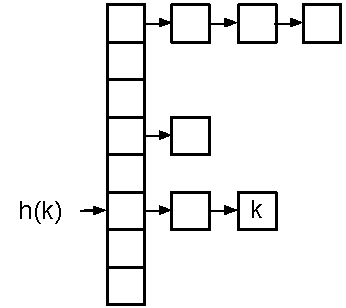
\includegraphics[scale=.75]{hash-tables/separate-chaining} &
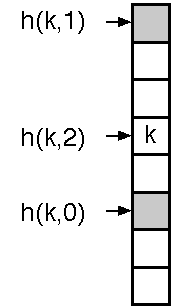
\includegraphics[scale=.75]{hash-tables/open-addressing} &
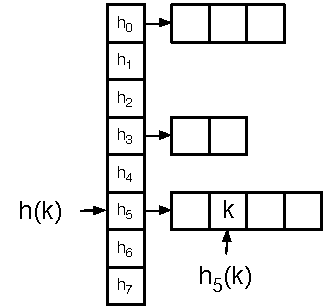
\includegraphics[scale=.75]{hash-tables/perfect-hashing} &
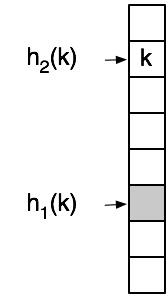
\includegraphics[scale=.75]{hash-tables/cuckoo-hashing} \\
separate chaining & open addressing & perfect hashing & cuckoo hashing
\end{tabular}
\end{center}
\end{example}
We will consider the first two in this lecture.

In our discussion, we will assume we have a set of $n$ keys $K$ that
we want to store and a hash function $h : \cname{key} \rightarrow [0,
  \ldots, m-1]$ for some $m$.


\section{Separate Chaining}

In 15-122 you studied hash tables using separate chaining.  As you may
recall, the idea is to maintain an array of linked lists.  All keys
that hash to the same location (bin) in the sequence are maintained in
a linked list.  To find a key a key $k$, go to the location $h(k)$,
and search the list belonging to that location for that key.  To
insert a key, first try to find the key.  If the key is in the list, then
possibly replace it with the new value (depending on the semantics of
insert), otherwise add the key to either the start or the end of the
list.

\begin{exercise}
Write pseudocode for inserting to, searching from and deleting from a
separate chaining hash table.
\end{exercise}

The costs of these operations is related to the average length of a
chain, which is $n/m$ when there are $n$ keys in a table with $m$
chains. We call $\lambda = n/m$ the \emph{load factor} of the table.

When searching for a key the key might or might not be in the table.
We refer to the two cases as a \emph{successful search} and an
\emph{unsuccessful search}, respectively.  Assuming that
we can compute $h(k)$ in $O(1)$ work, we then have:

\begin{claim} 
For simple uniform hashing, an \emph{unsuccessful search} takes
expected $\Theta(1 + \lambda)$ work.

\begin{proof} The average length of a list is $\lambda$.  If we search
  for a key that is not in the table, we need to search the whole list
  to determine the key is not in the table.  Including the cost of
  computing $h(k)$, the total work is $\Theta(1 + \lambda)$.
\end{proof}
\end{claim}

\begin{claim} For 
simple uniform hashing, a \emph{successful search}
takes expected $\Theta(1 + \lambda)$ work.

\begin{proof} 
To simplify the analysis, we assume that keys are added at the end of
the chain\footnote{The average successful search time is the same
  whether new keys are added to the front of the end of the
  chain.}. The cost of a successful search is the same as an
unsuccessful search at the time the key was added to the table.  That
is, when we first insert a key, the cost to insert it is the same as
the cost of an unsuccessful search.  Suppose this cost is $T_k$.
Subsequent searches for this key is also $T_k$.  When the table has
$i$ keys, the cost of inserting a new key is expected to be $(1 +
i/m)$.  Averaging over all keys, the cost of a successful search is
\[\frac1{n} \sum_{i=0}^{n-1} (1 + i/m) = \frac1n(n+n(n-1)/(2m)) = 1 + (n-1)/(2m) \leq 1 + \lambda/2
= \Theta(1+\lambda) \]
\end{proof}
\end{claim}

That is, for successful searches we examine half the list on average
and unsuccessful searches the full list.  If $n = O(m)$ then with
simple uniform hashing, all operations have expected $O(1)$ work and
span.  Even more importantly, some chains can be long, $O(n)$ in the
worst case, but it is expectation they will have length $\lambda$.
The advantage of separate chaining is that it is not particularly
sensitive to the size of the table.  If the number of keys is more
than anticipated, the cost of search becomes only somewhat worse. If
the number is less, then only a small amount of space in the table is
wasted and the cost of search is faster.

\section{Open Address Hash Tables}

The next technique does not need any linked lists but instead stores
every key directly in the locations of an array, which we will refer
to as cells.  Open address hashing using so-called linear probing has
an important practical advantage over separate chaining: it causes
fewer cache misses since typically all locations that are checked are
on the same cache line.

The basic idea of open addressing is to maintain an array that is some
constant factor larger than the number of keys and to store all keys
directly in this array.  Every cell in the array is either empty or
contains a key.

To decide to which cells to assign a key, open addressing uses an
ordered sequence of locations in which the key can be stored.  In
particular let's assume we have a function $h(k,i)$ that returns the
$i^{th}$ location for key $k$.  We refer to the sequence
\[\cseq{h(k,0), h(k,1), h(k,2), \ldots}\] as the \emph{probe} sequence.
We will get back to how the probe sequence might be assigned, but
let's first go through how these sequences are used.  When inserting a
key the basic idea is to try each of the locations in order until we
find a cell that is empty, and then insert the key at that location.
Sequentially, insert would look like:

\begin{algorithm}[Insertion into an Open Address Hash Table]~
\begin{lstlisting}
function insert$(T,k)$ = let
  function insert'$(T,k,i)$ =
    case $T[h(k,i)]$ of
      None => update$(T,h(k,i),k)$
    | Some($k'$) => 
        if $(k = k')$ then $T$
        else insert'$(T,k,i+1)$
in insert'$(T,k,0)$ end
\end{lstlisting}
\end{algorithm}

\begin{example}
Suppose the hash table has the following keys:
\begin{center}
\begin{tabular}{l c c c c c c c c }
         & 0 & 1 & 2 & 3 & 4 & 5 & 6 & 7 \\ \cline{2-9}
  T = &    &  B &    &    & E & A &    & F \\\cline{2-9}
\end{tabular}
\end{center}
Now if for a key $D$ we had the probe sequence $\cseq{1, 5, 3,
  \cdots}$, then we would find location 1 and 5 full (with $B$ and
$E$) and place $D$ in location 3 giving:
\begin{center}
\begin{tabular}{l c c c c c c c c }
      & 0 & 1 & 2 & 3 & 4 & 5 & 6 & 7 \\ \cline{2-9}
  T = &   & B &   & D & E & A &   & F \\ \cline{2-9}
\end{tabular}
\end{center}
\end{example}

Note that for the update operation to be constant work and span, $T$
must be a single threaded array.  Also, the insertion algorithm will
loop forever if all locations are full.  Such an infinite loop can be
prevented by ensuring that $h(k,i)$ tries every location as $i$ is
incremented, and checking when the table is full.  Also, as described,
the algorithm will insert the same key multiple times over.  This
problem is easily corrected by checking if the key is in the table and
if so returning immediately.

To search we have the following code:

\begin{algorithm}[Find in an Open Address Hash Table]~
\begin{lstlisting}
function find$(T,k)$ = let
  function find'$(T,k,i)$ =
    case $T[h(k,i)]$ of
      None => false
    | Some($k'$) =>
        if (k = k') then true
        else find'$(T,k,i+1)$@\vspace{.1in}@
in find'$(T,k,0)$ end
\end{lstlisting}
\end{algorithm}

\begin{example}
In the table 
\begin{center}
\begin{tabular}{l c c c c c c c c }
      & 0 & 1 & 2 & 3 & 4 & 5 & 6 & 7 \\ \cline{2-9}
  T = &   & B &   & D & E & A &   & F \\ \cline{2-9}
\end{tabular}
\end{center}
if key E has the probe sequence $\cseq{7, 4, 2, \cdots}$,
\cname{find}$(T,\mbox{E})$ would first search location 7, which is full,
and then location 4 where it finds E.
\end{example}

\begin{question}
What if we want to delete a key?
\end{question}

Let's say we deleted $A$ from the table
above, and then searched for $D$. Will \cname{find} locate it?  No, it will
stop looking once it finds the empty cell where $A$ was. One solution
might be to rehash everything after a delete.  But that would be an extremely
expensive operation for every delete. An alternative is to use what is
called a \emph{lazy delete}.  Instead of deleting the key, simply
replace the key with a special \cname{Hold} value.  That is, introduce
an entry data type:

\begin{lstlisting}[numbers=none]
datatype $\alpha$ entry = Empty | Hold | Full of $\alpha$
\end{lstlisting}
\begin{question}
How do we change \cname{find} and \cname{insert} to handle
\cname{Hold} entries?
\end{question}
For \cname{find}, simply skip over a \cname{Hold} entry and move to
the next probe.  $\cname{insert}(v)$ can replace the first
\cname{Hold} entry with $\cname{Full}(v)$.  But if \cname{insert}
needs to check for duplicate keys, it first needs to search for the
key. If it finds the key it overwrites it with the new
value. Otherwise it continues until it finds an empty cell, at which
point it can replace the first \cname{Hold} in the probe sequence.

The main concern with lazy deletes is that they effectively increase the
load factor, increasing the cost of the hash table operations. If the
load factor becomes large and performance degrades, the solution is to
rehash everything to a new larger table.  The table should be a
constant fraction larger each time the table grows so as to maintain
amortized constant costs.

Now let's consider some possible probe sequences we can use.  Ideally,
we would like a key to use any of the possible $m!$ probe sequences
with equal probability.  This ideal is called \emph{uniform
  hashing}. But uniform hashing is not practical. Common probe
sequences, which we will consider next, are
\begin{itemize}
\item linear probing
\item quadratic probing
\item double hashing
\end{itemize}

\subsection{Linear Probing}

In linear probing, to insert a key $k$, it first checks $h(k)$ and
then checks each following location in succession, wrapping
around as necessary, until it finds an empty location.  That is, the
$i^{th}$ probe is \[h(k,i) = (h(k) + i) \mod m.\]  Each position
determines a single probe sequence, so there are only $m$ possible
probe sequences.

\begin{question}
What are some advantages and disadvantages of linear probing?
\end{question}

The problem with linear probing is that keys tend to cluster.  It
suffers from \emph{primary clustering}: Any key that hashes to any
position in a cluster (not just collisions), must probe beyond the
cluster and adds to the cluster size.  Worse yet, primary clustering
not only makes the probe sequence longer, it also makes it
more likely that it will be lengthen further.

What is the impact of clustering for an unsuccessful search? Let's
consider two extreme examples when the table is half full,
$\lambda=1/2$ (or equivalently, $m = 2n$).  Clustering is minimized
when every other location in the table is empty.  In this case, the
average number of probes needed to insert a new key $k$ is $3/2$: One
probe to check cell $h(k)$, and with probability $1/2$ that cell is
full and it needs to look at the next location which, by construction,
must be empty.  In the worst case, all the keys are clustered, let's
say at the end of the table. If $k$ hashes to any of the first $n$
locations, only one probe is needed.  But hashing to the $n^{th}$
location would require probing all $n$ full locations before finally
wrapping around to find an empty location.  Similarly, hashing to the
second full cell, requires probing $(n-1)$ full cells plus the first
empty cell, and so forth.  Thus, under uniform hashing the average
number of probes needed to insert a key would be

\[1 + [n + (n-1) + (n-2) + .... + 1]/m = 1 + n(n+1)/2m  \approx n/4 \]

Even though the average cluster length is 2, the cost for an
unsuccessful search is $n/4$. In general, each cluster $j$ of length
$n_j$ contributes $n_j(n_j+1)/2$ towards the total number of probes
for all keys.  Its contribution to the average is proportional the
$\emph{square}$ of the length of the cluster, making long cluster
costly.

We won't attempt to analyze the cost of successful and unsuccessful
searches, as considering cluster formation during linear probing is
quite difficult. We make the following claim:

\begin{claim} When using linear probing in a hash table of size $m$
that contains $n = \lambda m$ keys, the average number of probes needed
for an unsuccessful search or an insert is
\[\frac12\left(1 + \frac1{(1-\lambda)^2}\right) \]
and for a successful search is
\[\frac12\left(1 + \frac1{1-\lambda}\right). \]
\end{claim}

As you can see from the following table, which shows the expected
number of probes under uniform hashing, the performance of linear
probing degrades significantly when the load factor increases:

\begin{tabular}{l r r r r r}
\toprule
$\mathbf{\lambda}$    & 1/4 & 1/2 & 2/3 & 3/4 & 9/10 \\ \midrule
\textbf{successful}  & 1.2 & 1.5 & 2.0 & 3.0 &  5.5 \\
\textbf{unsuccessful}& 1.4 & 2.5 & 5.0 & 8.5 & 50.5 \\
\bottomrule
\end{tabular}

Linear probing is quite competitive, though, when the load factors are
in the range 30-70\% as clusters tend to stay small. In addition, a
few extra probes is mitigated when sequential access is much faster
than random access, as in the case of caching.  Because of primary
clustering, though, it is sensitive to quality of the hash function or
the particular mix of keys that result in many collisions or clumping.
Therefore, it may not be a good choice for general purpose hash
tables.

\subsection{Quadratic Probing}

Quadratic probe sequences cause probes to move away from clusters, by
making increasing larger jumps. The $i^{th}$ probe is
\[ h(k,i) = (h(k) + i^2) \mod m.\]

\begin{question}
What are some advantages and disadvantages of quadratic probing?
\end{question}

Although, quadratic probing avoids primary clustering, it still has
\emph{secondary clustering}: When two keys hash to the same location,
they have the same probe sequence. Since there are only $m$ locations
in the table, there are only $m$ possible probe sequences.

One problem with quadratic probing is that probe sequences do not
probe all locations in the table. But since there are $(p+1)/2$
quadratic residues when $p$ is prime, we can make the following
guarantee.

\begin{claim} If $m$ is prime and the table is at least half empty, then
quadratic probing will always find an empty location. Furthermore, no locations
are checked twice.

\newcommand{\ceiling}[1]{\lceil #1 \rceil}
\begin{proof} (by contradiction)
Consider two probe locations $h(k) + i^2$ and $h(k) + j^2, 0 \leq i,j
< \ceiling{m/2}$. Suppose the locations are the same but $i \neq j$. Then
\begin{align*}
h(k) +i^2 &\equiv (h(k) + j^2)\mod m \\
i^2 &\equiv j^2 \mod m \\
i^2 - j^2 &\equiv 0 \mod m \\
(i-j)(i+j) &\equiv 0 \mod m
\end{align*}
Therefore, since $m$ is prime either $i-j$ or $i+j$ are divisible by
$m$. But since both $i-j$ and $i+j$ are less than $m$, they cannot be
divisible by $m$.  Contradiction.

Thus the first $\ceiling{m/2}$ probes are distinct and
guaranteed to find an empty location.
\end{proof}
\end{claim}

Computing the next probe is only slightly more expensive than linear
probing as it can be computed without using multiplication:
\begin{align*}
h_i - h_{i-1} &\equiv (i^2 - (i-1)^2)\mod m \\
h_i &\equiv (h_{i-1} + 2i - 1) \mod m
\end{align*}

Unfortunately, requiring that the table remains less than half full
makes quadratic probing space inefficient.

\subsection{Double Hashing}


Double hashing uses two hash functions, one to find the initial
location to place the key and a second to determine the size of the
jumps in the probe sequence.
The $i^{th}$ probe is \[h(k,i) = (h_1(k) + i\cdot h_2(k)) \mod
m.\]
Keys that hash to the same location, are
likely to hash to a different jump size, and so will have different
probe sequences.  Thus, double hashing avoids secondary clustering by
providing as many as $m^2$ probe sequences.

How do we ensure every location is checked? Since each successive
probe is offset by $h_2(k)$, every cell is probed if $h_2(k)$ is
relatively prime to $m$. Two possible ways to ensure $h_2(k)$
is relatively prime to $m$ are, either make $m=2^k$ and design $h_2(k)$
so it is always odd, or make $m$ prime and ensure $h_2(k) < m$. Of
course, $h_2(k)$ cannot equal zero.

Double hashing behaves quite closely to uniform hashing for
careful choices of $h_1$ and $h_2$. Under uniform hashing the
average number of probes for an unsuccessful search or an insert is at most
\[1 + \lambda + \lambda^2 +... = \left(\frac1{1-\lambda}\right) \]
and for a successful search is at most
\[\frac1{\lambda} \left (1+\ln \biggl(\frac1{1-\lambda}\biggr)\right). \]

The former bound is because the probability of needing more than $i$
probes is at most $\lambda^i$. A search always needs one probe, and with
probability $\lambda$ needs a second probe, and with probability
$\lambda^2$ needs a third probe, and so on.  The bound for a
successful search for a key $k$ follows the same probe sequences as
when it was first inserted. So if $k$ was the $(j+1)^{th}$ key inserted
the cost for inserting it is at most $1/(1-j/m)$.  Therefore
the average cost of a successful search is at most
\begin{align*}
\frac1{n} \sum_{j=0}^{n-1} \frac{1}{1-j/m} &=
\frac{m}{n}\sum_{j=0}^{n-1} \frac{1}{m-j} \\
&=\tfrac1{\lambda}\left(\sum_{j=0}^{m} \frac{1}{j} + \sum_{j=0}^{m-n} \frac{1}{j}\right)\\
&= \tfrac1{\lambda}(H_m - H_{m-n}) \\
&\leq \tfrac1{\lambda}(\ln m + 1 - \ln(m-n)) \\
&= \tfrac1{\lambda}\Bigr(1+\ln \Bigl(\tfrac1{1-\lambda}\Bigr)\Bigr)
\end{align*}


The table below shows the expected number of probes under the
assumption of uniform hashing and is the best one can expect by open
addressing.

\begin{tabular}{l r r r r r r}
\toprule
$\mathbf{\lambda}$    & 1/4 & 1/2 & 2/3 & 3/4 & 9/10 \\ \midrule
\textbf{successful}  & 1.2 & 1.4 & 1.6 & 1.8 & 2.6 \\
\textbf{unsuccessful}& 1.3 & 2.0 & 3.0 & 4.0 & 10.0 \\
\bottomrule
\end{tabular}

Comparing these numbers with the numbers in the table for linear
probing, the linear probing numbers are remarkable close when the load
factor is 50\% or below.

\begin{question}
What are some advantages and disadvantages of double hashing?
\end{question}

The main advantage with double hashing is that it allows for smaller
tables (higher load factors) than linear or quadratic probing, but at
the expense of higher costs to compute the next probe.  The higher
cost of computing the next probe may be preferable to longer probe
sequences, especially when testing two keys equal is expensive.

\section{Hash Table Summary}

Hashing is a classic example of a space-time tradeoff: increase the
space so table operations are faster; decrease the space but table
operations are slower.

Separate chaining is simple to implement and is less sensitive to the
quality of the hash function or load factors, so it is often the
choice when it is unknown how many and how frequently keys may be
inserted or deleted from the hash table.  On the other hand open
addressing can be more space efficient as there are no linked lists.
Linear probing has the advantage that it has small constants and works
well with caches since the locations checked are typically on the same
cache line. But it suffers from primary clustering, which means its
performance is sensitive to collisions and to high load factors.
Quadratic probing, on the other hand, avoids primary clustering, but
still suffers from secondary clustering and requires rehashing as soon
as the load factor reaches 50\%. Although double hashing reduces
clustering, so high load factors are possible, finding suitable pairs
of hash functions is somewhat more difficult and increases the cost of
a probe.

\section{Parallel Hashing}

\begin{question}
How can we parallelize open addressing?
\end{question}

In the parallel context, instead of inserting, finding or deleting one
key at a time, each operation takes a set of keys.  Since a hash
function distributes keys across slots in the table, we can expect
many keys will be hashed to different locations.  The idea is to use
open addressing in multiple rounds.  For \cname{insert}, each round
attempts to write the keys into the table at their appropriate hash
position.  For any key that cannot be written because another key is
already there, the key continues for another round using its next
probe location. Rounds repeat until all keys are written to the table.

In order to prevent writing to a position already occupied in the
table, we introduce a variant of the \cname{inject} function.
The function
\begin{lstlisting}[numbers=none]
injectCond$(I, S)$ : (int ** $\alpha$) seq ** ($\alpha$ option) seq -> ($\alpha$ option) seq
\end{lstlisting}
takes a sequence of index-value pairs
$\cseq{(i_1,v_1),\ldots,(i_n,v_n)}$ and a target sequence $S$ and
conditionally writes each value $v_j$ into location $i_j$ of $S$.  In
particular it writes the value only if the location is set to None. If
there are two or more values with the same index (a conflict) then it
conditionally writes the value only for the \emph{first} occurrence of
the index (recall that \cname{inject} uses the \emph{last} occurrence
of an index).  Resolving conflicts in \cname{injectCond} can be
implemented using a parallel primitive called
write-with-min\footnote{For more information, see the paper
  \emph{Reducing Contention Through Priority Updates} by Julian Shun,
  Guy Blelloch, Jeremy Fineman and Phillip Gibbons:
  \url{http://www.cs.cmu.edu/~jshun/contention.pdf}.}.

%%  and there is no previous equal index in $IV$.  That is,
%% it conditionally writes the value for the \emph{first} occurrence of
%% an index; recall

\begin{algorithm}[Parallel Insertion with Open Addressing]~
\begin{lstlisting}
function insert$(T, K)$ = let
  val $i$ = $0$
  while $(|K| > 0)$ with $(T,K,i)$
    val $I$ = $\cseq{(h(k,i),k) : k \in K}$
    val $T$ = injectCond$(I, T)$
    val $K$ = $\cseqf{k \in K}{T[h(k,i)] \neq \cname{Some}(k)}$
    val $i$ = $i+1$
in $T$ end
\end{lstlisting}
\end{algorithm}

For round $i$, \cname{insert} uses each key's $i^{th}$ probe in its
probe sequence and attempts to write the key to the table.  To see
whether it successfully wrote a key to the table, it reads the value
written to the table and checks if it is the same as the key. In this
way it can filter out all keys that it successfully wrote to the
table.  It repeats the process on the keys it didn't manage to write,
using the keys' $(i+1)$ probes.

\begin{example}
Consider a table with the following entries before
round $i$:
\begin{center}
\begin{tabular}{l c c c c c c c c }
      & 0 & 1 & 2 & 3 & 4 & 5 & 6 & 7 \\ \cline{2-9}
  $T$ = &   & A &   & B &   &   & D & C \\\cline{2-9}
\end{tabular}
\end{center}
If $K = \cseq{\mbox{E, F}}$, $h(\mbox{E},0) = 1$, and $h(\mbox{F},0) =
2$, then on the first round $I = \cseq{(1, \mbox{E}), (2, \mbox{F})}$ and the
\cname{injectCond} would fail to write $E$ to index $1$ but would
succeed in writing $F$ to index $2$ resulting in the following table:
\begin{center}
\begin{tabular}{l c c c c c c c c }
      & 0 & 1 & 2 & 3 & 4 & 5 & 6 & 7 \\ \cline{2-9}
  $T$ = &   & A & F & B &   &   & D & C \\\cline{2-9}
\end{tabular}
\end{center}
On the next iteration we have $K = \cseq{\mbox{E}}$ and $i = i+1 = 1$.
\end{example}

Note that if $T$ is implemented using a single threaded array, then
parallel \cname{insert} basically does the same work as the sequential
version adding the keys one by one. The only
difference is that the parallel version may add keys to the table in a
different order than the sequential.  

\begin{example}
With linear probing, the parallel version adds F first using 1 probe
and then adds E at index 4 using 4 probes:
\begin{center}
\begin{tabular}{l c c c c c c c c }
      & 0 & 1 & 2 & 3 & 4 & 5 & 6 & 7 \\ \cline{2-9}
  $T_P$ = &   & A & F & B & E &   & D & C \\\cline{2-9}
\end{tabular}
\end{center}
Whereas, the sequential version might add E first using 2 probes,
and then F using 3 probes:
\begin{center}
\begin{tabular}{l c c c c c c c c }
      & 0 & 1 & 2 & 3 & 4 & 5 & 6 & 7 \\ \cline{2-9}
  $T_S$ = &   & A & E & B & F &   & D & C \\\cline{2-9}
\end{tabular}
\end{center}
Both versions make $5$ probes in the table. 
\end{example}

Since we showed that, with suitable hash functions and load factors,
the expected cost of insert is $O(1)$, the expected work for the
parallel version is $O(|K|)$.  In addition, in each round, the
expected size of $K$ decreases by a constant fraction, so the span is
$O(\log |K|)$.

\begin{exercise}
Assuming uniform hashing and a hash table of size $2|K|$, prove that
the expected size of $K$ decreases by a constant fraction in each call
to \cname{insert'}.
\end{exercise}

\begin{exercise}
Describe how to do hash table searches in parallel and deletions in
parallel.
\end{exercise}

% How does a hash table implementation compare with a treap
% implementation of Set and Table?
% \begin{itemize}
%  \item search is faster (in expectation)
%   \item insert is faster (in expectation)
%   \item map, reduce, remain linear
%   \item union/merge is slower or faster depending on particular settings
% \end{itemize}

% We assume a function $\cname{injectCond}(IV, S) : (int \times \alpha)
% \cname{seq} \times (\alpha \cname{option}) seq \rightarrow (\alpha
% \cname{option}) seq$.  It takes a sequence of index-value pairs
% $\cseq{(i_1,v_1),\ldots,(i_n,v_n)}$ and a target sequence $S$ and
% conditionally writes each value $v_j$ into location $i_j$ of $S$.  In
% particular it only writes the value if the location is set to None and
% there is no previous equal index in $IV$.

% Note that if $T$ is implemented using single threaded arrays, then
% this basically does the same work as the sequential version adding the
% keys one by one.

\section{Comparison to Tree Tables}

\begin{question}
How does a hash table implementation compare with a tree table
implementation of Set and Table?
\end{question}

\begin{itemize}
\item Searches are faster in expectation
\item Insertions are faster in expectation
\item Map, reduce, and filter remain linear work
\item Union/merge can be slower.
\end{itemize}

\begin{question}
What does a tree table support efficiently that a hash table does not?
\end{question}

In contrast to a tree table, a hash table cannot support range queries
efficiently since it does not maintain any order on the keys.

\flushchapter
